\chapter{Literature survey on modular vessel platform automation}
%{Related work on modular vessel platform automation}
\label{LiteratureStudy}

% Link this chapter in the whole. Whats the role. 
This chapter summarizes literature relevant to automated vessel platforming systems to answer subquestion 1:
\begin{itemize}
	\item What is the state of the art within automated vessel platforming systems?
\end{itemize}

For effective discussion on ship automation good definitions of terminology are required to avoid misinterpretation. Definitions that are used in this work are described in section \ref{literatureDefinitions}, supplemented with various other common interpretations. 

This literature review shows various works on automated control of vessel platforming systems, yet it was noticed that the majority of relevant works focus on either the "assembly process" or "control of a platform with adaptable configuration", so they will be discussed in those groups in section \ref{literatureAutomatedAssemblySystems} and \ref{literatureConfigurationDependentControl} respectively. 

\citet{chen2020survey} provides an overview on cooperative control methods for waterborne transport where  vessel-to-vessel cooperation is classified in three categories; formation control, cooperative collision avoidance, and cooperative manipulation. Vessel platform motion control would fall into the category of cooperative manipulation (a fleet of vessels coordinate their actions to fulfill certain tasks\cite{chen2020survey}). Platform self assembly has facets overlapping with formation control (steering a group of vessels to form a specific geometric configuration and control their coordinated collective motion \cite{chen2020survey}) and cooperative manipulation of the multi-robot fleet. As sources that specifically describe modular vessel platforming systems are limited, so a broader range of works is discussed in this review, such as fields of cooperative manipulation, formation control, and reconfiguration automation from general robotic science. 

Discussed projects are schematically shown in section \ref{literatureConclusion}, where this chapter also elaborates on the resulting gap of knowledge that drives this paper. Various works that are introduced and discussed in this chapter are further used in chapter \ref{chap:sysAnalysis} to analyze system characteristics and discuss design choices and considerations of these projects.

%In the search for literature, the following keywords were used:Autonomy, automated, automation, smart ship, vessel, ship, self-assembly, assembly, platform, platforming

\section{Terminology}
\label{literatureDefinitions}
Definitions used to describe automation of various vessel processes differ a lot troughout the marine sector. Relevant terminology and their interpretation will be discussed here. 

\begin{itemize}
	\item \textbf{Automation} refers to the full or partial replacement of a function previously carried out by the human operator. This implies that automation is not all or none, but can vary across a continuum of levels, from the lowest level of fully manual performance to the highest level of full automation (definition according to \citet{parasuraman2000model}).
	
	\item \textbf{Control} is purposeful action on or in a process to meet specified objectives, which can be exercised by a human or by automation (defnition according to \cite{IMO103ISORegulatoryScopingExMass}). Control, pertaining to a ship, often primarily refers to the motion of the hull, altough other tasks (such as connecting in this paper) can refer to this as well.  
	
	\item \textbf{Modular reconfigurable robot} (MRR) systems are made up of many repeated modules (or units) that can be rearranged or can rearrange themselves into different configurations depending on the task the robot is to solve at the time (definition according to \citet{seo2019modular})
	
	\item \textbf{Configuration} in reconfigurable robotics is commonly generalized to incorporate the connectivity of the modules (which module is connected to which, represented as an adjacency matrix, a linked list, and the like) into the conventional robotics definition of the term that refers to just the pose of the robot (the full set of the joint angles of the	robot) (definition according to \citet{seo2019modular}).
	
	\item \textbf{Reconfiguration} is the process of changing connectivity \citet{seo2019modular}, which may include \textbf{assembly} and/or \textbf{disassembly}.
	
	\item \textbf{Vessel-platform}, or sometimes referred to as platform, is a combination of vessels, or  \textbf{modules} that are connected to form a floating structure.
	
	\item A \textbf{cybernetic} system is self-regulating. The term cybernetics was developed by Norbert Wiener in 1948 \citet{norbert1948or}. This regulation is done by the system according to a given (control) law. \citet {smithers1997autonomy} describes the difference between cybernetics and automation: " Cybernetic systems are thus self-regulating systems, systems that are not just able to move or to act by themselves but are also able to regulate and control their movements or actions so as to maintain their effectiveness in the face of disturbances and perturbations, according to some predefined control law or rule of regulation" 
	
	\item An \textbf{autonomous} system is considered self-governing, thus capable of constructing its own laws, according to \citet{smithers1997autonomy}. In practice the interpretation of "autonomous ship" differs among organisations, generally ranging from being interchangably used with "automated" or "cybernetic".  \citet{smithers1997autonomy} argues that the beforementioned definition is more consistent to use in other sciences while it also functions as an independant important concept; "Autonomous systems are different from cybernetic systems, and they form a more general class of self-regulating systems, those that form their own laws of regulation as well as regulate their behavior with respect to these self-made laws." Indiscriminate use of the term "autonomous" can cause confusion, misinterpretation and false expectations.  For further use in this paper, the term autonomous is avoided as it is deemed too ambiguous at this point and other terminology (cybernetics and automation) suffice.
	
	\item An \textbf{unmanned} surface vessel (USV) is a ship with no humans on board \cite{IMO103ISORegulatoryScopingExMass}. According to this definition being unmanned does not characterize the nature of the controller. The vessel can be controlled by a human, via remote control, or it can be machine controlled to meet its goals. 'Reduction of human presence' and 'reduction of human control' often go hand in hand \cite{heo2017analysis} but are not equal as can be seen from the example of remote-, human-controlled systems. 
	
	\item A ship's \textbf{power source} provides energy to fuel its actuators. There exists a trend in developing electric powered vehicles. Electrification of vehicle's power source is often done with climate influencing emmisions in mind. Vehicle power source, whether fueled by fossil fuels, electric or by other means has no direct influence on the degree of automation. Goals of automation and electrification often overlap, and there are some shared benefits, but they are distinct concepts. 
\end{itemize}

For further reading on definitions, interpretation, categorization and terminology, the following sources are recommended; \citet{vagia2016literature} discusses the evolution of use of 'levels of autonomy' and 'levels of automation' in robotics. It is shown how authors use terminologies and taxonomies in different ways. \citet{smithers1997autonomy}'s describes common use of terms "cybernetics", "automation" and "autonomy", and discusses ways of interpretation. 

The International Maritime Organisation (IMO) shows ongoing changes to the proposed definition of 'autonomy' in the contexts of shipping \citet{IMO103ISORegulatoryScopingExMass} in an effort to standardize usage. The last proposed definition of autonomy appears to mean something different than how it is used in other sciences such as philosophy, biology and psychology. How the marine sector started to adopt the word 'autonomy' and how the use will develop is unclear, but it will need a concrete definition of an overarching organisation such as IMO or ISO to avoid discussion. 

Use of the terminology: "unmanned surface vehicle" (USV) does not always capture the essence of projects that strive towards automation. The term USV could also contain vehicles that are human controlled from a distance by means of remote control. For control purposes it might be more suitable to categorize according to the nature of the controller (human controlled, machine controlled or hybrid), instead of whether there are humans on board or not. 

It is found that when discussing "vessel automation", various topics can stay especially vague. The following questions are considered key to get insights on  a so called 'automated vessel system':
\begin{itemize}
	\item \textbf{What functions are exactly automated?} Generally the main function of a vessel is considered movement, thus the motion control is often seen as the main function. Other tasks such as power management (e.g., fueling), system health monitoring, maintenance or on-board activities could also be implied to  all be automatic on an 'automated ship', although they are often not. Environmental awareness is likely neccesary for vessel automation on busy waterways, as the ship needs to take other entities into account to safely perform its voyage, although not a requirement for basic motion control. 
	\item \textbf{To what degree are these functions automated?} One automated vessel might be to only able to control its position to a reference given by an operator, while more advanced systems equipped with a planning and guidance layer might be able to plan and control a trajectory through dynamic waterways. Various categorizations of automation and autonomy exist, each with their own purpose and complexity, of which many are compared in \citet{vagia2016literature}, for the interested reader.
\end{itemize}

For a history lesson and some fundamentals about vessel control theory, consider reviewing \citet{clarke2003foundations}.
For a regulatory flavour of challenges for vessel automation consider consulting \citet{komianos2018autonomous} as the author examines operational, regulatory and quality assurance challenges due to development and deployment of autonomous vessels. Many projects that work on automated, unmanned or autonomous vessels are summarized, of which most are specifically aiming at deployment at sea. Existing regulations where adaptation is deemed required to allow further ship automation are being discussed. Specific comments about required regulatory changes are discussed on: the Convention of life at sea (SOLAS), the International Convention on Standards of Training, Certification and Watchkeeping for Seafarers (STCW), the Convention on the International Regulations for Preventing Collisions at Sea (COLREG), the International Convention for the Prevention of Pollution from Ships (MARPOL), the International Convention on Maritime Search and Rescue (SAR). Various  interpretations of autonomy and resulting characteristics are quoted, although no single definition is stated. Interpretation ranges from "unmanned" to "machine controlled".

\section{Automated reconfigurating vessel systems}
\label{literatureAutomatedAssemblySystems}

Two projects have been identified to build up the majority of the literature on automation of fleet assembly into floating structures. The first discussed works are on a project that developed a nameless fleet of container-like modules with rope and hook connectors, while the second works are developed in the "Roboat" project with vessels of similar naming. 

%% Container-like fleet
\citet{o2014self} and \citet{paulos2015automated} record developments of their fleet of container-like modules. The vessels are rectangles with dimentions of the same ration of standard shipping containers, but at a model scale (Fig. \ref{fig:o2014selfModuleDesign}). The specific shape is aimed to demonstrate how an upscaled system could be rapidly deployed from standard container carriers. 

% Example bridge
\citet{o2014self} greatly illustrates potential of modular marine structures to solve logistical challenges by forming a bridge that allowed crossing of a remote controlled toy car (figure \ref{fig:o2014selfBridge}). The structure formed consists of partially functioning modules in between. Which functions were active on these modules is not mentioned. It is expected that connection systems were functional on all vessels, while other functions, such as positioning, were active on a part of the fleet. 
 
 \begin{figure}[h!]
	\centering
	\makebox[\textwidth][c]{
		\begin{minipage}{0.45\textwidth}
			\centering
			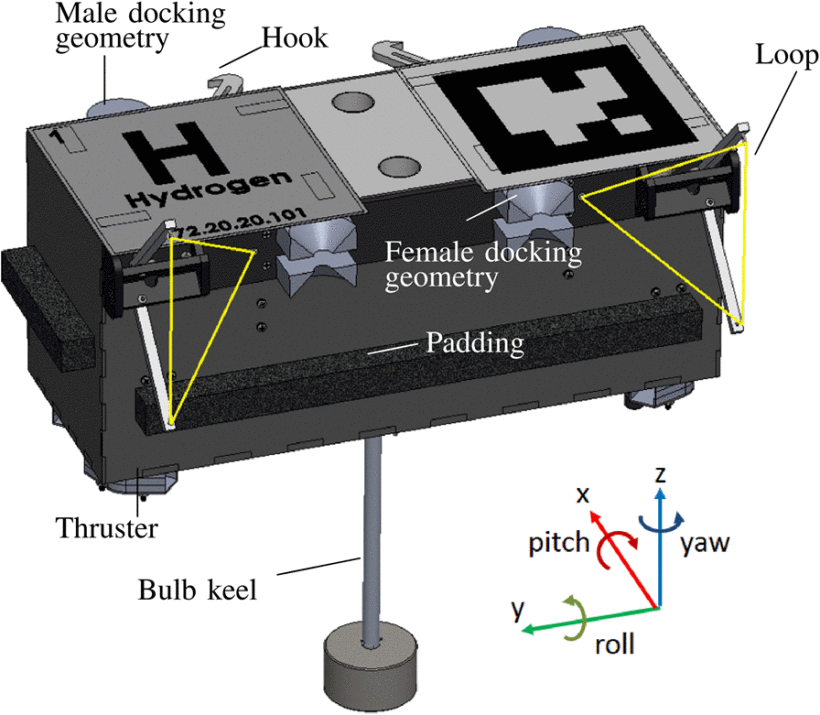
\includegraphics[width=0.95\textwidth]{img/o2014selfModuleDesign}
			\caption{Container-like platform module used in \cite{o2014self} and \cite{paulos2015automated}}
			\label{fig:o2014selfModuleDesign}
		\end{minipage}\hfill
		\begin{minipage}{0.45\textwidth}
			\centering
			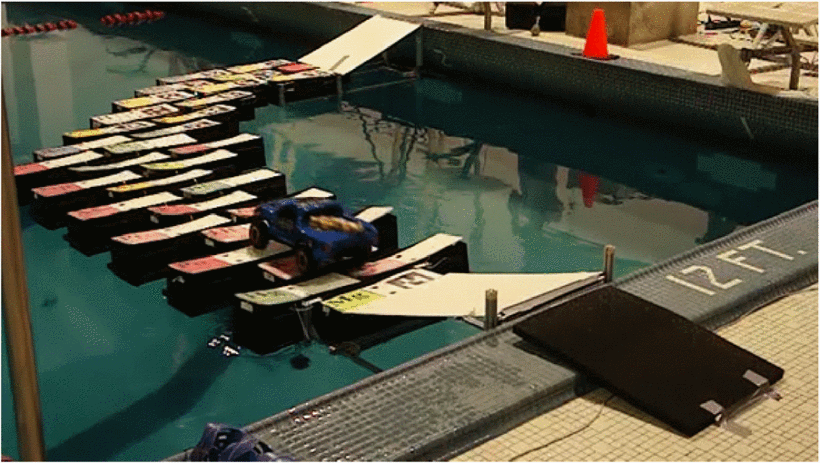
\includegraphics[width=0.95\textwidth]{img/o2014selfBridge}
			\caption{Static floating structure formed from 33 modules \cite{o2014self}}
			\label{fig:o2014selfBridge}
		\end{minipage}
	}
\end{figure}

% Roboat
The Roboat project aims to develop a floating combined infrastructure from modules which are also reffered to as 'Roboats', where the main collaborators are Massachusetts Institute of Technology (MIT) and the Amsterdam institute for Advanced Metropolitan Solutions (AMS). \citet{wang2018design} initially presents the Roboat system equipped with a real-time nonlinear model predictive control system. The vessel design has four thrusters configured in a cross to produce holonomic motions. The design is based to form a framework upon which further tests can be performed for transportation and self-assembly to floating infrastructures. This paper is the first published document on development of the "Roboat" concept, while the project  aims to scale up from model vessels to full scale operation \cite{roboatWebsite}. Early scale up is shown in \citet{wang2020roboat} to a 1.0x2m version at solo operation. All following resources that use Roboat equipment are however based on the smaller models. 

\begin{figure}[h!]
	\centering
	\makebox[\textwidth][c]{
		\begin{minipage}{0.45\textwidth}
			\centering
			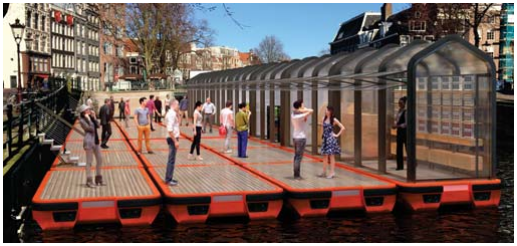
\includegraphics[width=0.95\textwidth]{img/roboatStructureConcept}
			\caption{Roboat's concept of creating floating structures from square modules \citet{wang2018design}.}
			\label{roboatStructureConcept}
		\end{minipage}\hfill
		\begin{minipage}{0.45\textwidth}
			\centering
			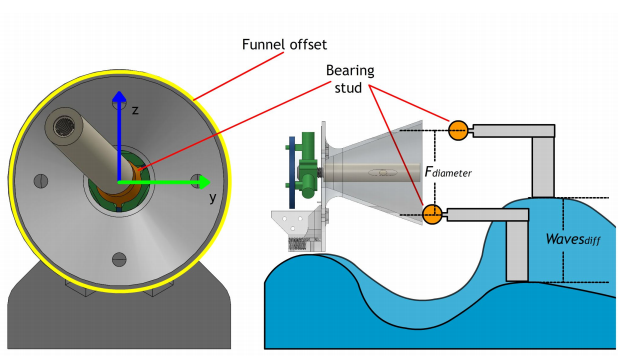
\includegraphics[width=0.95\textwidth]{img/roboatLatchingBallcone}
			\caption{ \citet{mateos2019autonomous} shows a ball and funnel connection mechanism tested on Roboat vessels.}
			\label{roboatLatchingBallcone}
		\end{minipage}
	}
\end{figure}

\citet{mateos2019autonomous} shows development of a latching system consisting of male/female ball/cone components. This paper discusses latching hardware and shows experimental results of a vessel system that performs platform assembly with the implemented latching hardware.

\citet{8901099} and \citet{kelly2019algorithms} present trajectory planning algorythms for reconfiguration of modular surface structure components. The proposed core logic of the shapeshifting algorythm is in finding the largest overlap between current and desired configuration. Overall phases of the proposed reconfiguration scheduler are shown in figure \ref{fig:kelly2019algorithms_statemachine_schematic}. \citet{8901099} show approaches and experimental results of platform shapeshifting, by distincting the whole reconfiguration problem into task planning, trajectory planning and trajectory tracking (see Fig. \ref{fig:roboatreconfigurationplanning}). 

\begin{figure}[H]
	\centering
	\makebox[\textwidth][c]{
		\begin{minipage}{0.45\textwidth}
			\centering
			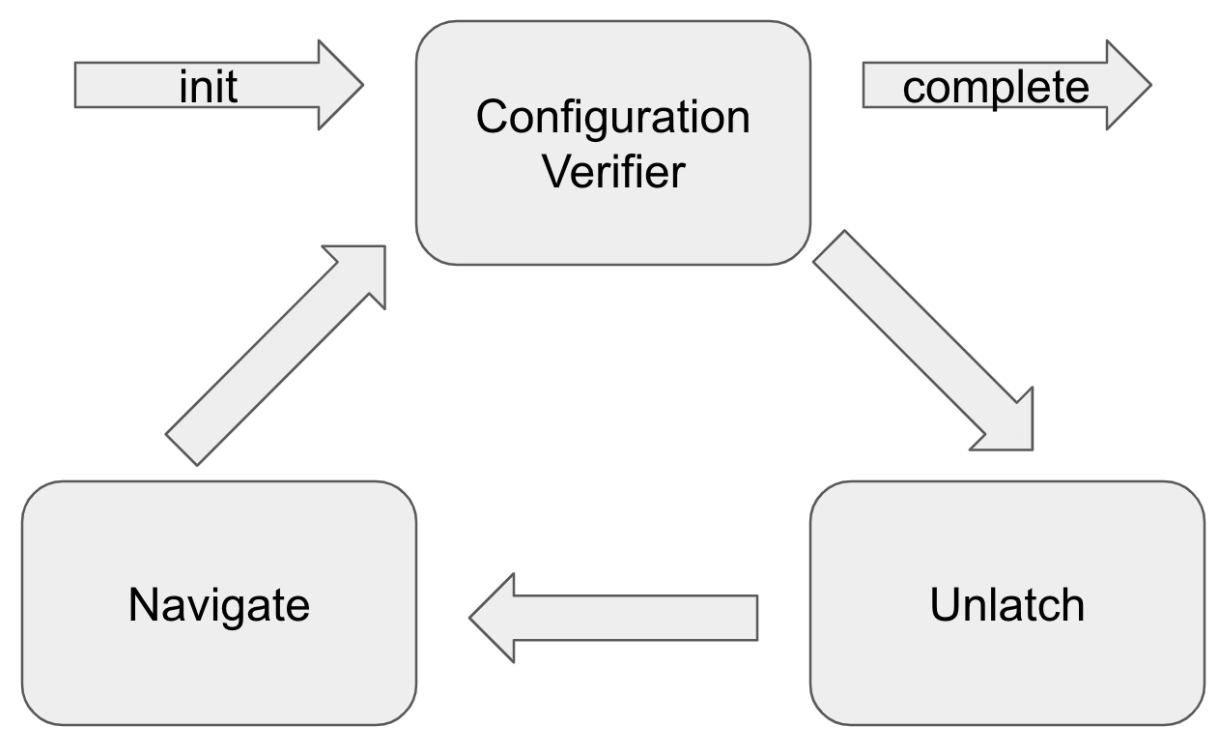
\includegraphics[width=0.95\textwidth]{img/kelly2019algorithms_statemachine_schematic}
			\caption{Platform reconfiguration system phases from \citet{kelly2019algorithms}}
			\label{fig:kelly2019algorithms_statemachine_schematic}
		\end{minipage}\hfill
		\begin{minipage}{0.45\textwidth}
			\centering
			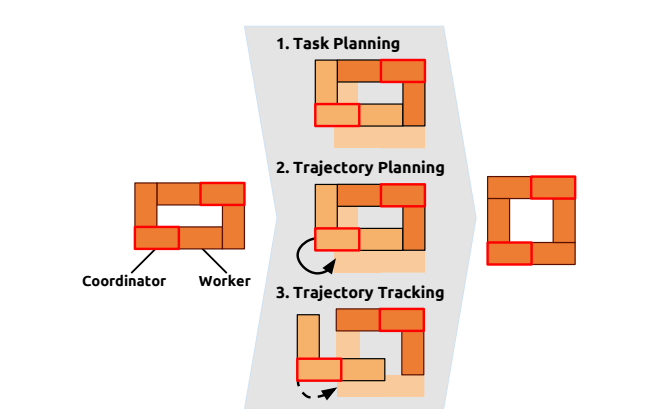
\includegraphics[width=0.95\textwidth]{img/RoboatReconfigurationPlanning}
			\caption{Shapeshifting process of \citet{8901099} in Three Stages: 1) Task Planning finds
				a decomposition for unlatching into two assemblies and relatching
				them in a desired shape. 2) Trajectory Planning computes a
				trajectory for one assembly from one latching point to another one.
				3) Trajectory Tracking controls the assembly along the trajectory. }
			\label{fig:roboatreconfigurationplanning}
		\end{minipage}
	}
\end{figure}

The literature on non-maritime multi robot assembly proved to be more expansive, thus readers are encouraged to take a further look at this if they are interested to get inspired from a broader body of literature. Two of such works on assembly of general robotic systems are as follows.

\citet{tuci2018cooperative} describes key literature on assembly of multi-robot systems. The author noticed the pattern in studies that gave reason to distinct three physical connection strategies in multi-agent systems: Pushing only, grasping, and caging. This reseach had no focus on vessels or orher marine applications, but describes many great works from a broader, general robotics body of literature. 

\citet{miyashita2008morphology} shows the relation between morphology on the success of assembly in the eventually desired shape of stochastic robots. This work took inspiration from biological examples of self-assembly to design and build a water-based modular robotic system consisting of plastic tiles capable of aggregation on the water surface. An externally applied electric potential controlled the self-assembly of the aggregates. This paper is particularly interesting as it shows a completely different approach (stochastic vs deterministic) and operational scale than the container like modules and the Roboat project, illustrating the vast amount of possible solutions to self-assembly challenges. 

\section{Collaborative motion control}
\label{literatureConfigurationDependentControl}

As arbitrary shaped waterborne structures are formed, it can be beneficial to be able to manipulate motion of the combined body. This section discusses works that focus on cooperative manipulation of waterborne objects. Modular strucures are of particular interest, although works describing motion control of such systems are limited. The majority of the encountered literature focusses on controlling motion of a single large object  (e.g. a large unactuated barge) by utilizing combined effort of  a fleet of automated vessels (e.g. tugboats). 

\citet{johansen2013control} distincts three levels of hierarchy for motion control of over-actuated systems, as shown in Fig. \ref{johansen2013controlDistinction}. A high level motion control system generates virtual control efforts to meet control objectives. A second system allocates the desired virtual control effort between actuators, possibly taking into account issues such as actuator saturation and meeting secondary objectives such as power efficiency optimization. A third layer operates on the level of a single actuator such that it meets allocated state (e.g. propeller speed, actuator orientation). \citet{johansen2013control} provides a varied survey on control allocation algorithms from aerospace, maritime, automotive and mechatronic industries. Algorithms are classified in two main classes based on using linear or nonlinear models. 
	\begin{figure}[h]
		\centering
		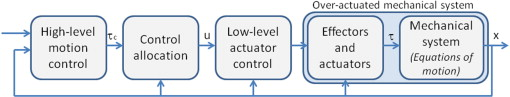
\includegraphics[width=0.7\textwidth]{ControlAllocationLoopExplained}
		\caption{\citet{johansen2013control} Control system structure including control allocation. The vector  denotes commanded virtual control effort (generalized forces), while  are the actual allocated control effort.}
		\label{johansen2013controlDistinction}
	\end{figure}
\citet{johansen2013control} mentions that the design on the control allocation algorithm and the high-level motion control algorithm cannot always be independent, and lack of feasibility of the control allocation should be observed and handled by the high-level motion control algorithm in order to avoid unacceptable degradation of performance in such cases. This division of the control system generally pertains a more common single vessel scenario, yet these principles are applied throughout the majority of multi-vessel scenarios as well. 

Various works describe different approaches for controlling motion of a larger vessel using a fleet of smaller modules (see 
\citet{feemster2006manipulation},\citet{4282954},  \cite{feemster2011comprehensive},  \citet{smith2007swarn}, \citet{bidikli2016robust}, \citet{esposito2008cooperative}, \citet{du2020cooperative},    
 and more). A generic usecase is motion of an uncontrolled ship with a fleet of small tugboats, as shown in Fig \ref{feemster2006manipulationExample}.  These works bear significant similarities with motion control of a modular platform, as both challenges are a form of collaborative manipulation. However, they differ as these works assume constant shape and dynamics of the controlled vessel. This often allows to reasonably assume that ship dynamics are known, which cannot easily be said for modular structures. A selection of these works that were found to illustrate a specific challenge or approach are briefly discussed. 
	
\begin{figure}[h!]
	\centering
	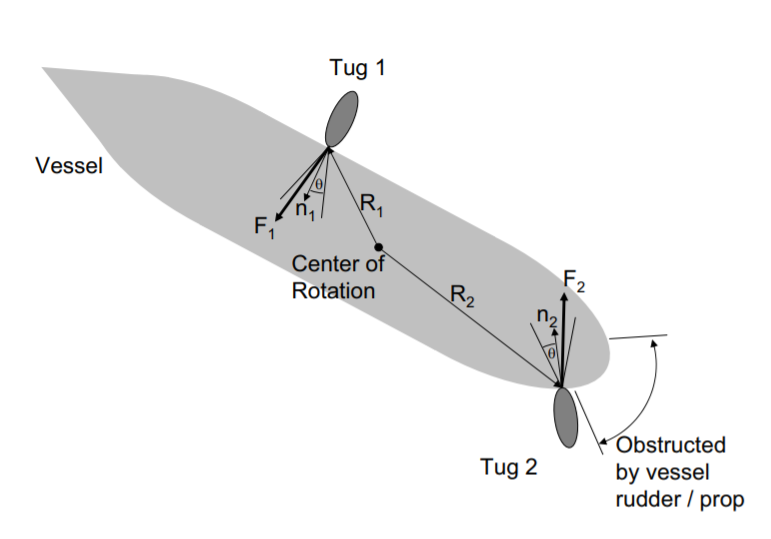
\includegraphics[width=0.5\textwidth]{feemster2006CollaborativeTugboat}
	\caption{Illustration of swarm forces on disabled vessel (\citet{feemster2006manipulation})}
	\label{feemster2006manipulationExample}
\end{figure}

\citet{feemster2006manipulation} considers the control problem of cooperative manipulation of a larger object by a team of smaller robotic vessels using a decentralized architecture. This work focusses on controlling only rotation, yet shows approaches and considerations to avoid a single point of failure from a centralized architecture. Other works also explore distributed control approaches, such as \citet{4282954},\citet{habibi2016distributed} and \citet{chen2019distributed}.

\citet{feemster2011comprehensive} presents a trajectory tracking framework of cooperative ship manipulation. Primary challenges are identified and described as: (1) the actuators are unidirectional and experience saturation; (2) the hydrodynamics of the system are difficult to characterize; and (3) obtaining acceptable performance under field conditions. An experimental setup shows a proposed control approach with separate trajectory generation, tracking control, and force allocation taking into account saturation of actuators. The controller employs an adaptive feedback law to compensate for unknown—difficult to measure—hydrodynamic parameters, employing a 3-DOF planar second order dynamical model. 

Various connection mechanisms are described in existing literature, each with different characteristics. \citet{smith2007swarn} investigates utilization of a swarm of automated tug boats to manipulate an object, where the tugboats are constrained to only exert a pushing force.  \citet{chen2019distributed} sheds light on contact dynamics in a cooperative manipulation challenge where tugboats can only exert pulling force, while also taking into account connector dynamics of an elastic towing line. 

\citet{bidikli2016robust} proposes an approach to control a large object with pushing tugboats, while his framework supports changing configuration as a novelty. The tugboats exert forces on the barge, and are treated as actuators of the large ship with time varying thruster-configuration. The controlled object is assumed under influence of hydrodynamic mass effects  and a self-tuning control gain strategy is employed. Efficiency of the presented controller is demonstrated trough simulation.

\citet{du2020cooperative} describes such a multi-vessel control architecture where tugboats are designed to satisfy allocated towing forces and angles. This formalized layers illustrate how tugboats effectively function as acuators with their own specific dynamics. This work is extended in \citet{du2021cooperative} to incorporate environmental disturbances. 

Contrary to previously mentioned works, \citet{park2019coordinated}  describes an approach of controlling a modular structure. The vessels that combine into the combined body are by themselves already fully actuated. The main control approach used is a PD controller to generate control effort, which is said be applicable to any configuration and reference. Allocating control effort between thrusters is implemented as an optimizer minimizing energy use to find actuator response. Experimental results show effectiveness of the proposed control strategy on three different configurations. 
The control system design is based on an approximate model, which scales according to a variable amount of vessels that are coneccted into the platform, but not to configuration shape. Translational inertia (directional dependent masses in x and y direction) is assumed to scale with $n$ amount of vessels, while rotational inertia was scaled quadratic by $n^2$. System inertia is represented by constant directional dependent mass as the sum of rigid body and hydrodynamic-added mass. 

\begin{figure}[h!]
	\centering
	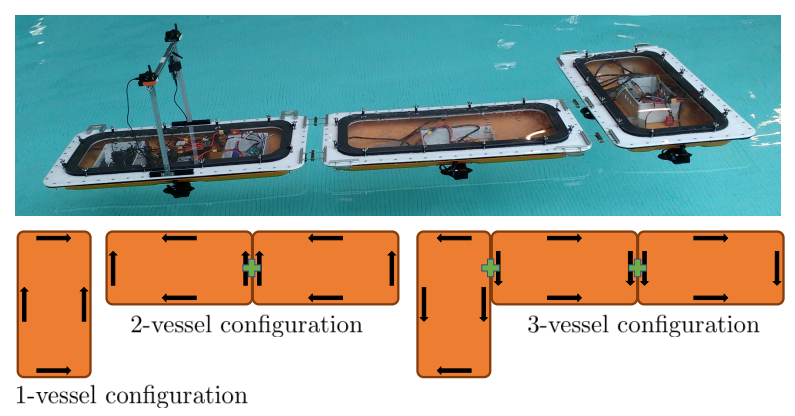
\includegraphics[width=0.6\textwidth]{park2019coordinatedConfigurations}
	\caption{ (Top) L-shape configuration of the connected-vessel platform and
		(Bottom) 3 different configurations used in the experiments. \citet{park2019coordinated}}
	\label{fig:park2019coordinatedConfigurations}
\end{figure}


\begin{figure}[h!]
	\centering
	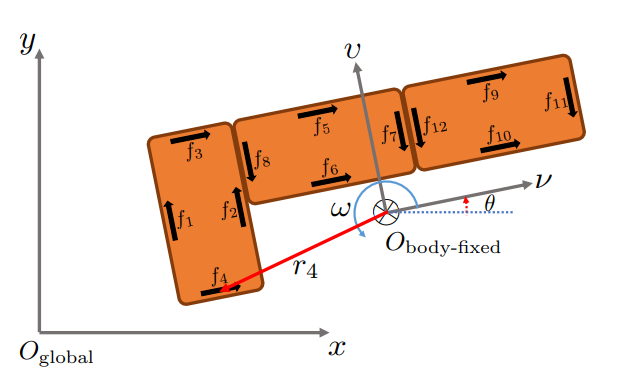
\includegraphics[width=0.5\textwidth]{park2019coordinatedBodyFrame2}
	\caption{An example of a rigid body of three connected vessels, where each black arrow drawn on the body of a vessel represents force exerted from a propeller. \citet{park2019coordinated}}
	\label{fig:park2019coordinatedBodyFrame}
\end{figure}

Scenarios where smaller vessels manipulate a significantly larger object, dynamics of the manipulators might be neglectible. However, assemblies with comparably sized modules will have rigid body dynamics affected by the configuration. \citet{park2019coordinated} distinguishes itself from the previously mentioned works as it attempts to predict dynamics of the assembly based on the configuration, albeit only on numbers and not on shape. \citet{park2019coordinated} proposes scaling rules to formulate the approximate platform model, as this is a key challenge that needs to be faced for model based controllers for modular strucures. 

\section{Gap in knowledge}
\label{literatureConclusion}
Works on modular vessel platform automation found through this literature survey originated from two project concepts; container shaped modules \cite{o2014self} shown in Fig \ref{fig:o2014selfModuleDesign} and Roboat \citet{wang2018design} shown in Fig \ref{roboatStructureConcept}). Contributions using Roboat vessels are credited to Advanced Metropolitan Solutions (AMS), Massachusetts Institute of Technology (MIT) or their collaboration. More literature exists on concepts that share similarities with vessel platform automation, but miss characteristics to classify as such. The majority of this relevant literature describe approaches for controlling a non-modular object using a fleet of smaller automated vessels. 

The discussed projects have a variety of works that explore facets on vessel platform automation, also showing many different design choices and approaches. Projects regarding automation of a multi-robot system performing reconfiguration or configuration dependent control are shown in table \ref{table:bigbadLiteratureSummary} to aid comparison. Works on multi-robot assembly and collaboration from aerospace and automotive branches have also been included in this schematic to give some perspective on developments in other fields. 

From this literature research it was concluded that no information is found of an modular fleet system that incorporates automated reconfiguration with collaborative configuration dependent control strategies in a single framework. Table \ref{table:bigbadLiteratureSummary} shows that works focus on either reconfiguration or collaborative control, not on combining the two, thus consequences of integrating the two behaviors in a single system are unmapped. Gathering and documenting approaches and experiences on integration can pave the road towards effective implementations to fully benefit from automated structure assembly while motion control of the combined platforms are enhanced by effective collaborative approaches. 

\newpage
\begin{sidewaystable}

\footnotesize
\begin{tabular}{|l|l|l|l|l|l|l|l|l|}
	\hline	
	\textbf{Title} & \textbf{Author} & \textbf{Year} &\makecell{\textbf{Land,} \\ \textbf{naval or} \\ \textbf{aerial}} &  \makecell{\textbf{Simulation or} \\ \textbf{experimental}} & \makecell{\textbf{Automated} \\ \textbf{assembly}}  & \makecell{\textbf{Changing control} \\  \textbf{system during} \\ \textbf{operation}} & \makecell{\textbf{System is} \\ \textbf{config.} \\ \textbf{dependent}} & \makecell{\textbf{Controlled} \\ \textbf{object is} \\ \textbf{modular}}  \\ \hline	
		
	\makecell{Autonomous self-assembly\\  in swarm-bots} & \citet{gross2006autonomous} 	& 2006 	& Land     	& Both  	& Yes  	& No		& No & Yes	\\ \hline
	\makecell{Object transport by modular \\ robots that self-assemble}& \citet{gross2006object}& 2006& Land & Experiment & Yes  & Yes	& No   & Yes  \\ \hline
	\makecell{A novel autonomous self-assembly \\ distributed swarm flying robot}& \citet{wei2013novel}& 2013& Aerial + land & Both& Yes& Yes& Yes &Yes\\ \hline
	\makecell{Self-assembly of a swarm of \\ autonomous boats into floating \\ structures}					& \citet{o2014self}        			& 2014     	& Naval                     	& Experiment             	& Yes                  & No         				& No      &Yes		\\ \hline
	\makecell{Automated Self-Assembly of Large \\  Maritime Structures by a Team of \\ Robotic Boats}		& \citet{paulos2015automated}        	& 2015     	& Naval                     	& Experiment             	& Yes                  & No         				& No      &Yes		\\ \hline
	\makecell{Cooperative Multi-Vessel Systems \\ for Waterborne Transport}                        				& \citet{chen2019cooperative}        	& 2019          & Naval                     	& Simulation                &  No               	& No         				& No   	&No	\\ \hline
	\makecell{Coordinated Control of a Reconfigurable \\ Multi-Vessel Platform: Robust Control \\Approach}     	& \citet{park2019coordinated}        	& 2019    	& Naval                  	& Both       			&  No                	& No                        		& Yes         &Yes 	\\ \hline
	\makecell{Autonomous latching system for \\robotic boats}     										& \citet{mateos2019autonomous}       & 2019    	& Naval                  	& Experiment			&  Yes                	& No                        		& No        &Yes  	\\ \hline
	\makecell{Trajectory Planning for the  \\ Shapeshifting of Autonomous Surface Vessels}     										& \citet{8901099}       & 2019    	& Naval                  	& Experiment			&  Yes                	& No                        		& No     &Yes     	\\ \hline
	\makecell{Algorithms for planning and \\ executing multi-roboat shapeshifting}     										& \citet{kelly2019algorithms}       & 2019    	& Naval                  	& Experiment			&  Yes                	& No                        		& No       &Yes  	\\ \hline
	\makecell{	Manipulation of large objects by swarms\\
		 		of autonomous marine vehicles. Part \\ 
		 		1-Rotation} 	& \citet{feemster2006manipulation}       & 2006    	& Naval                  	& Neither			&  Noy 	&  No 	&  Yes  & No \\ \hline
	\makecell{Positioning of Large Surface \\ Vessels using Multiple Tugboats} 	& \citet{4282954}       & 2007    	& Naval  	& Simulation		&   No  	& No 	&  Yes & No \\ \hline
	\makecell{Comprehensive framework for tracking control\\ and thrust allocation for a highly overactuated \\ autonomous surface vessel} 	& \citet{feemster2011comprehensive}       & 2011    	& Naval 	& Experiment		&  No 	& No	& Yes & No \\ \hline
	\makecell{Swarn Manipulation Of An Unactuated \\ Surface Vessel} 	& \citet{smith2007swarn}       & 2007    	& Naval & Simulation			&  No 	& No & Yes & No \\ \hline
	\makecell{Robust dynamic positioning of surface \\ vessels via multiple unidirectional \\ tugboats} 	& \citet{bidikli2016robust}   & 2016& Naval& Simulation	&  No 	& No & Yes & No \\ \hline
	\makecell{Cooperative manipulation on the water \\ using a swarm of autonomous tugboats} 	& \citet{esposito2008cooperative}& 2008& Naval & Experiment&  No &  No & Yes & No \\ \hline
	\makecell{Distributed model predictive control for\\ cooperative floating object transport \\ with multi-vessel systems} & \citet{chen2019distributed}& 2019 & Naval& Simulation	& No & No& Yes & No  \\ \hline
	\makecell{Cooperative control of autonomous tugs \\ for ship towing} 	& \citet{du2020cooperative}& 2020& Naval&Simulation& No& No & Yes& No \\ \hline 
\end{tabular}
\caption{Comparison of various projects related to vessel platform self assembly and/or collaborative platform motion control}
\label{table:bigbadLiteratureSummary}
\end{sidewaystable}

\newpage


